% Ich teile hier einfach mal meine Erfahrung der letzten Stunde trouble shooting.
% Latex = alles gut
% Bibtex = Denk einfach nich daran Umlaute zu benutzen. Nicht in der Bibliography, und auch nicht in Dateinamen
% Im eigentlichen Text gehts. Sachen wie Carrá sind aus irgendeinem Grund wiederum erlaubt, auch in der Bibliography
% Fix: {\"o} statt ö etc. (inkl. eckigen Klammern)

\chapter{Einführung}

Dieses Dokument, welches die Ausarbeitung zum Thema \glqq DevOps\grqq\ im Modul Software-Entwicklungsprozesse darstellt, stellt am Anfang die herkömmliche Unternehmenskultur und ihre Vor- sowie Nachteile dar. Im Zuge dieser Vorstellung wird dem Leser klar, warum diese Unternehmenskultur auf mittelfristige Sicht nicht funktionieren kann und zu Problemen führt. Als eine mögliche Lösung für diese Probleme wird dann das Konzept der \ac{DevOps}-Philosophie vorgestellt. Hierzu wird zuerst kurz der Ursprung des \ac{DevOps} aufgezeigt, danach werden die Leitsätze und wichtigsten Prinzipien erklärt sowie auch einige Kritikpunkte an \ac{DevOps} beschrieben und abgehandelt.\\
Im nächsten Schritt wird ein grundsätzliches Modell vorgestellt, das Helfen kann, den Übergang von einer herkömmlichen Unternehmenskultur hin zu \ac{DevOps} zu bewerkstelligen. Außerdem werden auch einige Schritte genannt, die kontinuierlich vollzogen werden müssen, um \ac{DevOps} effizient gestalten zu können.\\
Am Ende der Ausarbeitung wird ein kleines Bild der realen Welt in der Industrie gezeichnet, z. B. wie weit \ac{DevOps} verbreitet ist bzw. warum es nicht genutzt wird usw.

\section{Herkömmliche Unternehmenskultur}



\section{Wall of Confusion}

\begin{itemize}
\item Wie funktionieren Unternehmen und Prozesse aktuell?
\item Wie sieht die typische Unternehmenskultur aus und welche Nachteile bringt sie mit sich? (vllt auch Vorteile, weil mir wollen ja sachlich ran gehen)
	\begin{itemize}
	\item Silodenken
	\item Wall of Confusion
	\end{itemize}
\item Warum braucht es etwas Neues?
\item (optional) Andere Ansätze die das selbe Problem angegangen sind (bzw. andere Modelle für Unternehmenskultur)?
\end{itemize}

\begin{figure}[h]
\centering
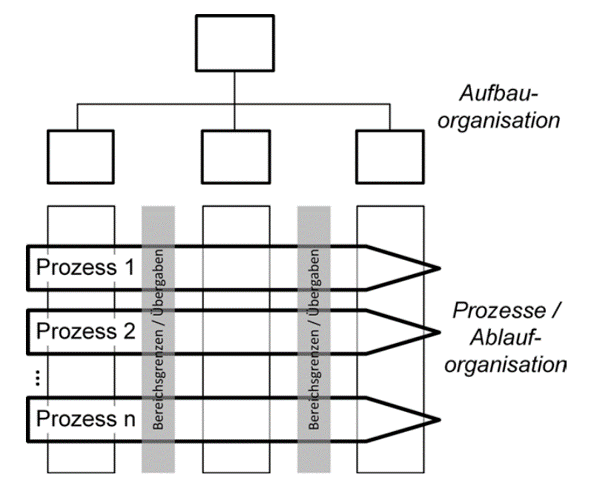
\includegraphics[width=0.7\textwidth]{Graphics/silodenken}
\caption{Silodenken \cite{halstenberg:2020}}
\end{figure}

\begin{figure}[h]
\centering
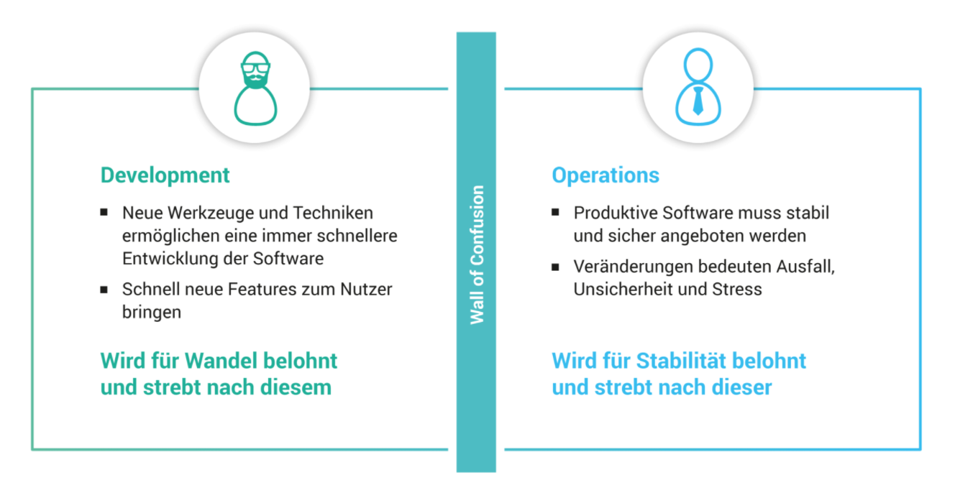
\includegraphics[width=0.8\textwidth]{Graphics/wall_of_confusion}
\caption{Wall Of Confusion \cite{novatec:2021}}
\end{figure}
